There are a number of underlying assumptions that permit finite-horizon optimal control techniques to be useful.

\begin{itemize}
	\item The mathematical dynamics accurately models the actual physical system being controlled.
	\item The current state of the system is known.
	\item The future state of the system can be accurately predicted as a function of the applied control.
\end{itemize}

Under an idealized simulation, these conditions are met by assuming perfect knowledge of initial and boundary conditions, and validating performance against using forward simulation identical to the controller's assumed model. In application, the above conditions will not be met exactly due to model inaccuracy, sensor noise, and prediction error. Thus, when applying control policies generated from optimal control procedures in noisy environments, one would expect the future physical state to diverge from that predicted from the controller's model, and thus a degradation in the performance of the controller.

This stems from optimal control being an \emph{open loop} control method, where the error in the state estimation is not observed as the physical system evolves. Alternatively, \emph{closed loop} controllers~\cite{Papageorgiou1991,Papamichail} incorporate the state estimation at frequent intervals (e.g. less than one minute for freeway systems), and choose a control policy which is optimal for only the \emph{next} time-step. Such schemes are also referred to as \emph{reactive} schemes, which react to real-time conditions rather than attempt to anticipate future road conditions (predictive schemes).

\begin{figure}[htbp]
	\centering
	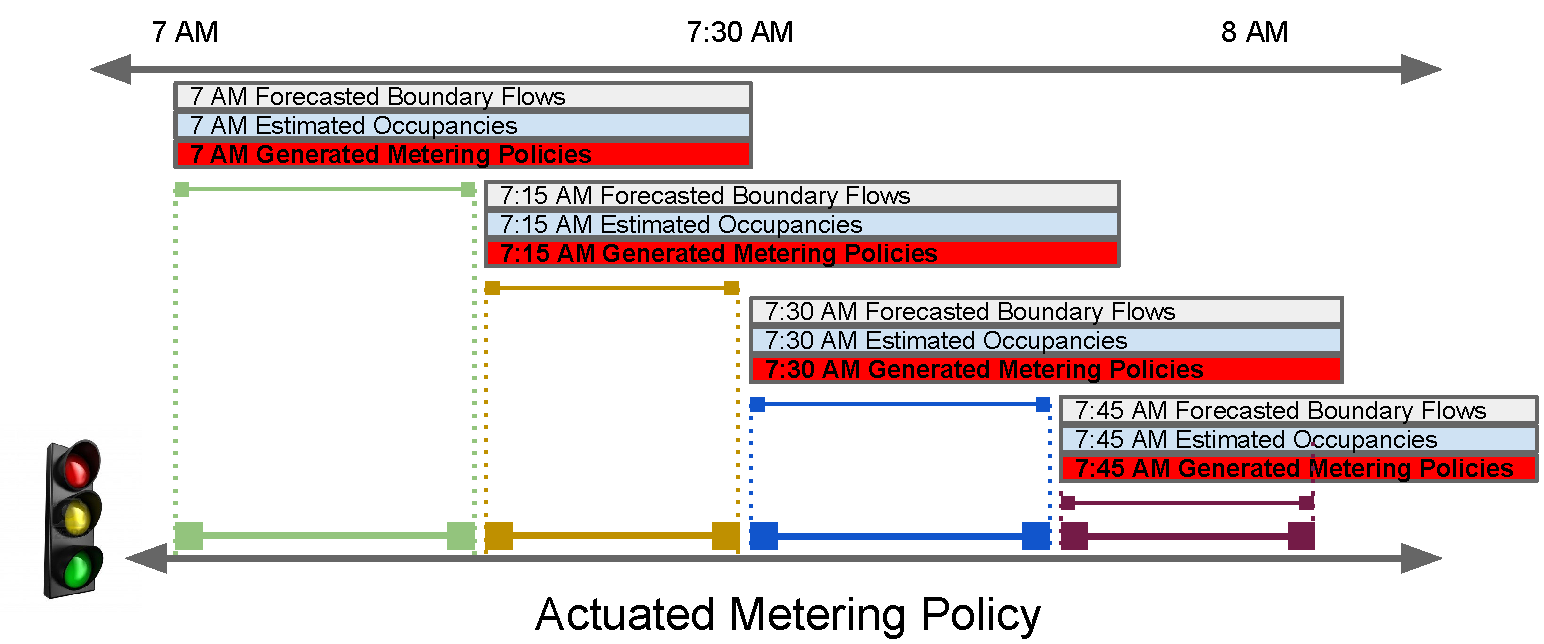
\includegraphics[width=\textwidth]{diagrams/mpc}
	\caption{Diagram of rolling-horizon MPC. At 15 minute intervals ($T_{\text{update}} =15$ minutes), the MPC controller requires an estimate of the current traffic (i.e. initial conditions) as well as predictions over the next 30 minutes ($T_{\text{horizon}} = 30$ minutes) for the future vehicle demands on the on ramps (i.e. boundary conditions).
	}
	\label{fig:mpc-overview}
\end{figure}

\emph{Model predictive control} (MPC) is a control technique which leverages the predictive benefits of optimal control approaches without the drawbacks of open loop control. At time instances occurring with an update period $T_{\text{update}}$, the MPC controller constructs an optimal control problem for the time period between the current time $t$ and some future time $t + T_{\text{horizon}}$, where $T_{\text{horizon}}$ is typically much larger than $T_{\text{update}}$ in order to properly leverage the predictive nature of optimal control. A new control policy is produced for the time period of the current optimal control problem, and the new control policy is then applied to the physical system. After $T_\text{update}$ time has elapsed, an updated control policy will be generated which leverages the newest available initial and boundary conditions. Given that $T_\text{update} < T_\text{horizon}$, the updated policy will be generated before the previous policy is completely applied, at which point the old control policy is discarded in favor of the new policy.


This process is summarized in Figure~\ref{fig:mpc-overview}. An MPC-based controller was implemented within the Connected Corridors system, leveraging the adjoint framework inside the optimal control problem. Numerical results with respect to adjoint control are given in Sections~\ref{sec:numerical-results-adjoint} and~\ref{sec:numerical_results-admm}.
